\documentclass[12pt]{report}
\makeindex

\usepackage{amsmath, amsfonts, amssymb, amstext, amscd, amsthm, makeidx, graphicx, hyperref, url, enumerate, mathabx, bbm}
\allowdisplaybreaks

\setcounter{chapter}{0}
\topmargin -.75in
\textheight 9.25in
\oddsidemargin 0.0in
\textwidth 6.5in

\newcommand{\al}{\alpha}
\newcommand{\be}{\beta}
\newcommand{\ga}{\gamma}
\newcommand{\ov}{\overline}
\newcommand{\ep}{\epsilon}
\newcommand{\N}{\mathbb N}
\newcommand{\C}{\mathbb C}
\newcommand{\R}{\mathbb R}
\newcommand{\Z}{\mathbb Z}
\newcommand{\Q}{\mathbb Q}
\newcommand{\la}{\langle}
\newcommand{\ra}{\rangle}
\newcommand{\da}{\lambda}
\newcommand{\I}{\mathbb I}
\newcommand{\sP}{\mathcal P}
\newcommand{\ds}{\displaystyle}
\newcommand{\id}{\mathbbm{1}}
\newcommand{\inc}{\hookrightarrow}
\newcommand{\homm}{\simeq}
\newcommand{\til}{\widetilde}
\newcommand{\om}{\omega}
\newcommand{\defn}{\noindent\textbf{Defn:}}
\newcommand{\sA}{\mathcal A}
\newcommand{\sE}{\mathcal E}
\newcommand{\thm}{\noindent\textbf{Theorem:}}


\begin{document}
\begin{center}
\textbf{{\LARGE MATH 3B}  \hfill} Discussion Worksheet - Thursday, May 31\\

\end{center}

\noindent\textbf{Improper Integration:}
\vspace{-.1in}
\begin{itemize}

\item Recall, we say an integral \emph{converges} if $\ds \int_a^b f(x) \, dx = $

\item We say an integral \emph{diverges} otherwise. 

\vspace{-.25in}
\begin{center}
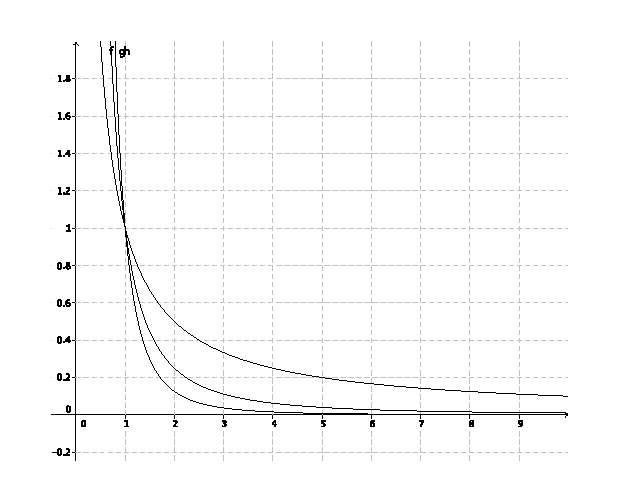
\includegraphics[scale=.95]{graphs.pdf}
\end{center}
\vspace{-.5in}

\noindent Examples:

\begin{itemize}

\item $\ds \int_1^\infty \frac1x \, dx = $

\medskip

\item $\ds \int_{1}^\infty \dfrac{1}{x^2} \, dx = $

\medskip

\item $\ds \int_{1}^\infty \dfrac{1}{x^3}\, dx = $

\end{itemize}
\end{itemize}

\noindent\textbf{FACTS and TESTS:}

\begin{itemize}

\item $p$\textbf{-Test}: If $a > 0$, then $\ds \int_a^\infty \dfrac{1}{x^p}$ is convergent for 

\bigskip

\item \textbf{Divergence Test:} If $f(x) \not\rightarrow 0$ as $x \to \infty$, then $\int_a^\infty f(x) \, dx$

\bigskip

\item \textbf{Comparison Test:} If $f(x) \geq g(x) \geq 0$ on $[a,\infty)$, then:

\begin{itemize}

\item if $\ds\int_a^\infty f(x) \, dx$ \hspace{1.5in}, then $\ds\int_a^\infty g(x) \, dx$


\item if $\ds\int_a^\infty g(x) \, dx$ \hspace{1.5in}, then $\ds\int_a^\infty f(x) \, dx$


\end{itemize}

\end{itemize}




\newpage


\noindent\textbf{Arc Length:} 


\begin{itemize}

\item If $f'$ is continuous on $[a,b]$, then the length of the curve $$\hspace{-1in}y=f(x), a \leq x \leq b \text{ is given by } L = $$



\item Strategies: %take it step by step (find y', square y', add 1, simplify/factor, then take sqrt and integrate)

\vspace{.75in}

\item Example: Find the length of the curve $y = \ln(\cos(x))$ where $0 \leq x \leq pi/3$

\vspace{1.5in}

\end{itemize}

\noindent\textbf{Surface Area:} 


\begin{itemize}

\item The surface area obtained by rotating the curve $y = f(x)$, $a \leq x \leq b$ about the $x$-axis is given by

\bigskip\bigskip

\item Where does this formula come from?

\vspace{1.75in}

\item If you're rotating about the $y$-axis, the curve is given as $x = g(y)$ from $c\leq y \leq d$ then the formula for surface area becomes

\bigskip\bigskip

\item Example: Write the formula that represents the area of the surface obtained by rotating the curve $y = e^x$, $1 \leq y \leq 2$ about the $y$-axis.

\end{itemize}




%\noindent\textbf{Problem 5:} Let $A= \left[ \begin{array}{rr} 1 & -3 \\ 3 & 5 \\ -1 & 7 \end{array} \right]$, ${\bf u} = \left[ \begin{array}{r} 2 \\ -1 \end{array} \right]$, and ${\bf b} = \left[ \begin{array}{r} 3\\ 2 \\ -5 \end{array} \right]$.
%
%\begin{itemize}
%
%\item[(a)] What is the domain and codomain of the transformation given by $T({\bf x}) = A{\bf x}$?
%
%\item[(b)] Find $T({\bf U})$, the image of ${\bf u}$ under the transformation $T$.
%
%\item[(c)] Find an ${\bf x}$ in $\R^2$ whose image under $T$ is ${\bf b}$.
%
%\item[(d)] Is there more than one ${\bf x}$ whose image under $T$ is ${\bf b}$.
%
%\end{itemize}

%
%\noindent\textbf{Problem 3:} Determine AS A GROUP whether or not the following statements are True or False and why:
%
%\begin{itemize}
%
%\item[1.] A basic variable in a linear system is a variable that corresponds to a pivot column in the coefficient matrix.
%
%\item[2.] If one row in an echelon form of an augmented matrix is $[ 0 \, 0 \, 0 \, 5 \, 0 ]$ then the associated linear system is inconsistent.
%
%\item[3.] Whenever a system has free variables, the solution set will have finitely many solutions.
%
%\item[4.] Another notation for the vector $\left[ \begin{array}{rr} -4 \\ 3\end{array} \right]$ is $[-4, \, 3]$. 
%
%\item[5.] An example of a linear combination of vectors ${\bf v_1}$ and ${\bf v_2}$ is the vector $\frac12 {\bf v_1}$.
%
%\end{itemize} 

%\medskip
%
%\noindent\emph{Proof of (i):} Let $f:A \to B$ be given as above. Then, for a regular value $y \in B$ of $f$, we have that $\ds \deg(f) = \sum_{x \in f^{-1}(y)} sgn(df_x)$ where $sgn(df_x) = 1$ if the isomorphism $df_x$ is orientation preserving and $-1$ if it is orientation reversing. Let $g:B \to C$ be another such map and let $y$ be a regular value of $g \circ f$. We have then that $d_f(x) \circ df_x$ is surjective for $x \in (g \circ f)^{-1}(y)$ so $dg_{f(x)}$ must be surjective which makes $y$ a regular value for $g$ as well. Since $A,B,$ and $C$ have the same dimension, $g^{-1}(y)$ is also a regular value of $f$ because were it not, $df_x$ would not be surjective which would imply $d_f(x) \circ df_x$ is not surjective which is not the case. Now, let $g^{-1}(y) = \{x_1, \dots, x_n \}$ and for each $x_i$, let $f^{-1}(x_i) = \{w_{i1}, \dots, w_{ik}\}$. For ease of notation, let $a_i = sgn(dg_{x_i})$, $b_{ij} = sgn(df_{w_{ij}})$ and then define $c_t = sgn(d(g\circ f)_{w_{ij}})$ for $1 \leq t \leq nk$. Since $$c_t = sgn(d(g\circ f)_{w_{ij}}) = sgn(dg_{x_i}\circ df_{w_{ij}}) = (sgn(dg_{x_i}))(sgn(df_{w_{ij}})) = a_ib_{ij}$$ we can conclude that $$\deg(g\circ f) = \sum_{t= 1}^{nk} c_t = \sum_{i = 1}^{n}\sum_{j=1}^k a_ib_{ij} = \left(\sum_{i = 1}^{n} a_i \right)\left(\sum_{j = 1}^{k} b_{ij} \right) = \deg(g)\deg(f).$$
%
%\medskip
%
%\noindent\emph{Proof of (ii):} Suppose that $f: A \to B$ as in (i) has $degree = 1$ and that the index $[\pi_1(B): f_\ast(\pi_1(A))] < \infty$. We know that for every subgroup $H < \pi_1(B)$, we are given a covering space $X$ such that $p_\ast(\pi_1(X)) = H$ where $p$ is a covering map. Thus, take $Y$ to be the covering space corresponding to $f_\ast(\pi_1(A))$. Thus, we have a lift $\til f: A \to Y$ such that $p \circ \til f = f$. Since $[\pi_1(B): f_\ast(\pi_1(A))] < \infty$ we can assume that $Y$ is an $n$-sheeted cover. We show that $\deg(p) = n$. Since $Y$ is an $n$-sheeted cover, we know that $p^{-1}(y)$ is a set containing $n$ points since the projection map $p$ is a local diffeomorphism. Thus, for each $x \in p^{-1}(y)$, we can arrange for $dp_x$ to be orientation preserving by giving $Y$ an orientation according to the isomorphism $dp_x$ on every sheet. Since $degree(f) = 1$, we have that $\deg(f) = \deg(p\circ \til f) = \deg(p)\deg(\til f) = 1$. So since $dp_x$ is orientation preserving and $\deg(p) \in \Z$, it must be that $\deg(p) = 1$ as well. This implies that $Y$ is a $1$-sheeted cover and thus, $[\pi_1(B): f_\ast(\pi_1(A))] =1$. Thus, $\pi_1(B) = f_\ast(\pi_1(A))$ and therefore, $f_\ast$ is surjective.
%
%\bigskip
%
%\noindent\textbf{2.} (i) Show that $M$ is simply connected. Prove that it is orientable.
%
%(ii) Prove that a connected Lie group is orientable. 
%
%(iii) Prove that a connected Lie group has Euler characteristic zero.
%
%\medskip
%
%\noindent\emph{Proof of (i):} Let $M$ be simply connected. We start by orienting $M$ along a path. Take $x \in M$ and give $T_x(M)$ an orientation. Then, since $M$ is connected, it is also path connected, so, for any $y \in M$ construct the path $p: [0,1] \to M$ with $p(0) = x$ and $p(1) = y$. Since $[0,1]$ is compact and $p$ is continuous, we know that $p([0,1])$ is compact. Now, for every $t \in [0,1]$ we can take parameterizations $U_t$ for each $p(t)$. By compactness, since $\{U_t\}$ covers $p([0,1])$, there exists a finite subcover, $\{U_k\}_{k=1}^n$ of $p([0,1])$. Since $p([0,1])$ is connected, we can arrange for our open cover to satisfy $U_i \cap U_{i+1} \neq \emptyset$ and can assume that $x \in U_1$ and $y \in U_n$. Now, for any $w \in U_1$, we give $T_w(U_1)$ the same orientation as $T_x(M)$. Since $U_i \cap U_{i+1} \neq \emptyset$, we can take a point in the intersection and continue to orient each point in each $U_i$ so that eventually, $T_y(M)$ has the same orientation as $T_x(M)$. 
%
%We now argue that our orientation does not depend on our path $p$. Let $q$ be another path connecting $x$ and $y$. Then, $p \homm q$. Thus, we can take the open cover given by $p$ and the open cover given by $q$ such that the covers intersect nontricially. Then, we can find a finite subcover such that the orientation of the finite subcover agrees with the orientation from both $p$ and $q$. This allows us to put an orientation on $T_x(M)$ for all $x \in M$ in a smooth way via our path giving us that $M$ is orientable. 
%
%\medskip
%
%\noindent\emph{Proof of (ii):} Suppose $G$ is a connected Lie group. We start similarly by letting $e \in G$ be the identity and giving $T_e(G)$. an orientation. Next, for a fixed $x \in G$, define $L_x: G \to G$ to be left multiplication by $x$; that is, $L_x(g) = xg$. Note that this is a diffeomorphism and therefore, $(dL_x)_e: T_e(G) \to T_x(G)$ is an isomorphism. Thus, given an ordered basis $\{v_\al\}$ of $T_e(G)$, we define a basis at $T_x(G)$ so be $\{(dL_x)_e(v_\al)\}$. Proceeding in this way for all $x \in G$ and using the fact that $L_x$ is smooth, we have that $G$ is orientable. 
%
%\medskip
%
%\noindent\emph{Proof of (iii):} Let $G$ be a connected Lie group. We were given in class that the Euler characteristic, $\chi(G)$, is equal to the Lefschetz number of the identity. Since Lefschetz number is a homotopy invariant (also proven in class), we can use the Lefschetz fixed point theorem conclude that $\chi(G) = 0$ if there is a map $f \homm \id$, the identity, where $f$ has no fixed points. Take $L_x$ defined in part (ii). Then, if $g \in G$ is a fixed point, we have that $L_x(g) = xg$ and therefore, $g = xg$. It follows then that $x = e$. This implies that for any nontrivial $x \in G$, $L_x$  has no fixed points. We show that $L_x \homm \id$. Since $G$ is connected, it is also path connected so let $p:[0,1] \to G$ be a path such that $p(0) = x$ and $p(1) = e$. Define now the map $F: G \times [0,1] \to G$ given by $F(g,t) = p(t)g$. Since multiplication is a smooth operation and $p$ is a path which is smooth, we have that $F$ is also smooth. Moreover, $$F(g,0) = p(0)g = xg = L_x(g) \, \text{ and } \, F(g,1) = p(1)g = eg = g = \id(g).$$ Since $L_x \homm \id$ and $L_x$ has no fixed points for a nontrivial $x$, we have that $\mathcal L(\id) = \mathcal L(L_x) = \chi(G) = 0$. 
%
%\bigskip
%
%\noindent\textbf{3.} Give a sketch of the construction of the Pontryagin manifolds. State the three main theorems and given an outline of the proof of one of them. 
%
%\medskip
%
%\noindent\emph{Proof:} We start by sketching the construction of a Pontryagin manifold. We start with a smooth map $f: M^m \to S^k$ where $M$ is a closed oriented $n$-manifold and $S^k$ the $k$-sphere. We then take $y \in S^k$ to be a regular value. Given a basis for $T_y(S^m)$ we can find a framing for $f^{-1}(y)$ given by a basis for $T_x(f^{-1}(y))^\perp$ for each $x \in f^{-1}(y)$. Letting $\nu$ be the framing we get by pulling back the above basis gives us a framed submanifold $(f^{-1}(y), \nu)$ which we refer to as the Pontryagin manifold of $f$. 
%
%The three main theorems are as follows:
%
%\begin{itemize}
%
%\item[Thm A:] Up to framed cobordism, the construction of a Pontryagin manifold is independent of choice of regular value and basis. 
%
%\item[Thm B:] $f$ is smoothly homotopic to $g$ if and only if the Pontryagin manifold of $f$ is framed cobordant to the Pontryagin manifold of $g$.
%
%\item[Thm C:] Every framed submanifold N of $M$ is a Pontryagin manifold of some map $f: M \to S^k$. 
%
%\end{itemize}
%
%We outline a proof for Theorem A in what follows. Let $f: M \to S^k$ be as given above and take $y \in S^k$ to be a regular value. Take $\{v_i\}_{i = 1}^k$ and $\{v'_i\}_{i=1}^k$ be basis for $T_y(S^k)$. We know that these bases are related via some matrix in $GL_n(\R)$ and thus there exists a path connecting this matrix to the identity. We can then define our framed cobordism by looking at the pulled back framing from this path applied to our basis. 
%
%Next, we showed that our construction is locally constant via a lemma that said we can take a neighborhood of $y$ such that for any regular value $z$ in the neighborhood of $y$, $f^{-1}(y)$ is framed cobordant to $f^{-1}(z)$. The proof of this used a family of rotations of the sphere connecting the identity and this regular value $z$ to build a cobordism.
%
%We made use of another lemma that says two smoothly homotopic maps that both have a regular value $y$ have Pontryagin manifolds that are framed cobordant. This implies that we can intersect the above neighborhoods so that our smooth homotopy gives a framed cobordism.
%
%Finally, taking two regular values $y$ and $z$ of $f$ we know that there is a family of rotations of the sphere that takes $y$ to $z$, call it $r$. Since $f$ is smoothly homotopic to $r \circ f$, we have that $f^{-1}(y)$ and $f^{-1}(r^{-1}(y)) = f^{-1}(z)$ are framed cobordant by what was argued above.






















\end{document}